\documentclass[xcolor={usenames,dvipsnames}, aspectratio=169, 12pt]{beamer}
\usetheme{tum}

\usepackage[T1]{fontenc}
\usepackage[english]{babel}
\usepackage{amsmath}
\usepackage{emojione}
\usepackage{wasysym}
\usepackage{calc}
\usepackage{xcolor}
\usepackage{tikz}
\usetikzlibrary{positioning, calc, fit, arrows.meta}
\usepackage{listings}
\usepackage{pgfplots}
\usepackage[separate-uncertainty=true]{siunitx}
\usepackage{svg}

\sisetup{per-mode=fraction, exponent-product=\cdot}
\pgfplotsset{width=10cm, height=3cm, grid style = dotted, compat=1.16}

\textwidth15cm
\textheight23cm
\topmargin-1cm
%\oddsidemargin0.5cm
%\evensidemargin0.4cm
\oddsidemargin1cm
\evensidemargin0cm
\setlength{\headheight}{13.6pt}
%\frenchspacing

%\clubpenalty10000
%\widowpenalty10000
%\displaywidowpenalty=10000

%\sloppy
%\hbadness 10000
\renewcommand{\topfraction}{0.85}
\renewcommand{\textfraction}{0.1}
\renewcommand{\floatpagefraction}{0.75}
\renewcommand{\UrlFont}{\small\ttfamily}

\definecolor{dkgreen}{rgb}{0,0.6,0}
\definecolor{gray}{rgb}{0.5,0.5,0.5}
\definecolor{mauve}{rgb}{0.58,0,0.82}

\definecolor{vsClass}{RGB}{0,110,150}
\definecolor{vsType}{RGB}{0,0,255}
\definecolor{vsString}{RGB}{215,160,135}
\definecolor{vsComment}{RGB}{10,100,30}

\definecolor{tumblue}{RGB}{0,101,189}

% Accessible colors from https://www.idpwd.com.au/resources/style-guide/
\definecolor{color0}{RGB}{247,127,0}
\definecolor{color1}{RGB}{81,181,224}
\definecolor{color2}{RGB}{206,224,7}
\definecolor{color3}{RGB}{15,43,91}

\definecolor{textcolor0}{RGB}{0,0,0}
\definecolor{textcolor1}{RGB}{0,0,0}
\definecolor{textcolor2}{RGB}{0,0,0}
\definecolor{textcolor3}{RGB}{255,255,255}

\hypersetup{pdftitle={Master Thesis}, pdfauthor={Sebastian Neubauer}, pdfsubject={PGO on GPUs}}

\addbibresource{references.bib}

\crefname{lstlisting}{listing}{listings}
\Crefname{lstlisting}{Listing}{Listings}

\lstset{
  numbers=left,                   % where to put the line-numbers
  numberstyle=\tiny\color{gray},  % the style that is used for the line-numbers
  stepnumber=1,
  numbersep=5pt,                  % how far the line-numbers are from the code
%  backgroundcolor=\color{gray!35},
  showspaces=false,               % show spaces adding particular underscores
  showstringspaces=false,         % underline spaces within strings
  showtabs=false,
  frame=single,                   % adds a frame around the code
  rulecolor=\color{black},        % if not set, the frame-color may be changed
  tabsize=4,                      % sets default tabsize to 4 spaces
  captionpos=b,                   % sets the caption-position to bottom
  breaklines=true,                % sets automatic line breaking
  breakatwhitespace=false,
  language=C,
  keywordstyle=\bfseries\color{vsType},
  commentstyle=\itshape\color{vsComment},
  stringstyle=\color{vsString},
  keywordstyle=[2]{\color{vsClass}},
  escapechar=ß,
  basicstyle=\scriptsize,
  morekeywords={u32, __u32, __be32, __le32,
		u16, __u16, __be16, __le16,
		u8,  __u8,  __be8,  __le8,
		size_t, ssize_t}
}

\lstdefinestyle{mysh}{
  language   = {bash},
  moredelim  = **[is][\color{OliveGreen}]{+}{+},
  basicstyle = \scriptsize,
}

\newcommand\lsthl[1]{{\color{Cyan}#1}}

% kirschju's masm lstlisting
\lstdefinelanguage
   [x86_64]{Assembler}
   [x86masm]{Assembler}
   {keywords={mov, call, ret, xor, rep, int, loop, push, syscall, pop,
        cdqe, cqo, cmpsq, cmpxchg16b, jrcxz, lodsq, movsxd, sub, add,
        vxorpd, popfq, pushfq, scasq, stosq, iretq, rdtscp, swapgs, shl, jz,
        vmfunc, enter, leave},
    keywords=[2]{rax, eax, ax, ah, al,
           rdx, edx, dx, dh, dl,
     rcx, ecx, cx, ch, cl,
     rbx, ebx, bx, bh, bl,
     rsi, esi, si, sih, sil,
     rdi, edi, di, dih, dil,
     rsp, esp, sp, rbp, ebp, bp, rip, eip, ip,
                 r8, r8d, r8w, r8b, r9, r9d, r9w, r9b,
           r10, r10d, r10w, r10b, r11, r11d, r11w, r11b,
           r12, r12d, r12w, r12b, r13, r13d, r13w, r13b,
           r14, r14d, r14w, r14b, r15, r15d, r15w, r15b},
     keywords=[3]{db, section}
   }
\lstdefinelanguage[amdgpu]{Assembler}{
	keywords={v_cmp_neq_f32_e32, s_cbranch_execz, s_branch, s_endpgm, image_sample, s_and_saveexec_b64, s_waitcnt,
		s_or_b64, v_mov_b32_e32, v_mul_f32_e32},
	keywords=[2]{v, v0, v1, v2, v3, v4, s, s0, s1, s2, s3, s4, vcc, exec},
	keywords=[3]{vmcnt},
	comment=[l]{;}
}

\newcommand{\ftabwidth}{7cm}
\newcommand{\ftabinnerwidth}{10cm}
\newcommand{\thead}{\rowcolor{Dandelion}}
\newcommand{\todd}{\rowcolor{Dandelion!50}}
\newcommand{\teven}{\rowcolor{Dandelion!30}}
\newcommand{\colorbitbox}[3]{%
\rlap{\bitbox{#2}{\color{#1}\rule{\width}{\height}}}%
\bitbox{#2}{#3}}

\setlength{\unitlength}{18mm}
\newcommand{\blob}{\textcolor{Gray}{\rule[-.2\unitlength]{2\unitlength}{.5\unitlength}}}

\newcommand\rblob{\rightmark
\begin{picture}(0,0)
\put(1,-\value{section}){\blob}
\end{picture}}

\newcommand\lblob{%
	\begin{picture}(0,0)
	\put(-3,-\value{section}){\blob}
	\end{picture}%
\thepage}

% Header and footline
\clearpairofpagestyles
\KOMAoptions{
	headsepline=true,
	footsepline=true,
}
\setkomafont{pageheadfoot}{\sffamily}

\automark[section]{section}
% Outer in twoside, right in oneside
\ohead{\itshape \rblob}
\ofoot{\pagemark}

% Style for first section pages inherits default
\newpairofpagestyles[scrheadings]{sectionheading}{
	\KOMAoptions{headsepline=false}
	\ohead{\rblob}
}
\newpairofpagestyles[scrheadings]{appendix}{
	\ohead{\itshape Appendix}
}

% Reduce spacing before paragraph
\RedeclareSectionCommands[
	beforeskip=-1ex plus -1ex minus -0.2ex,
	afterskip=-1em,% works as horizontal skip of 1em
]{paragraph,subparagraph}

\newcommand\bigsection[1]{
  \newpage
  %\cleardoublepage
  \thispagestyle{sectionheading}
  \vspace*{4cm}
  \section{#1}
  \vspace*{0.5cm}
  \pagestyle{scrheadings}
}

\addtokomafont{section}{\Huge}
\addtokomafont{subsection}{\Large}

\newcommand{\opt}[2]{#1}%
\newcommand{\de}[1]{}%
\newcommand{\en}[1]{#1}%
\newcommand{\code}[1]{\texttt{#1}}
\newcommand{\red}[1]{\textcolor{red}{#1}}
\makeglossaries{}

\algblockdefx[If]{If}{EndIf}[0]{\textbf{if}}{}
%Defines the alternative ending \Then to the \If command,
%which in turn ends in \EndThen
\algcblockdefx[Then]{If}{Then}{EndThen}{\textbf{then}}{\textbf{end if}}

\DeclareSIUnit\request{R}
\DeclareSIUnit\mips{MIPS}
\DeclareSIUnit\crypt{C}
\DeclareSIUnit\iteration{I}

%% https://tex.stackexchange.com/questions/55068/is-there-a-tikz-equivalent-to-the-pstricks-ncbar-command
\tikzset{
	ncbar angle/.initial=90,
	ncbar/.style={
	to path=(\tikztostart)
		-- ($(\tikztostart)!#1!\pgfkeysvalueof{/tikz/ncbar angle}:(\tikztotarget)$)
		-- ($(\tikztotarget)!($(\tikztostart)!#1!\pgfkeysvalueof{/tikz/ncbar angle}:(\tikztotarget)$)!\pgfkeysvalueof{/tikz/ncbar angle}:(\tikztostart)$)
		-- (\tikztotarget)
	},
	ncbar/.default=0.5cm,
}

\tikzset{square left brace/.style={ncbar=0.5cm}}
\tikzset{square right brace/.style={ncbar=-0.5cm}}

% https://tex.stackexchange.com/questions/75836/creating-a-seamless-xor-symbol-as-node
\tikzset{XOR/.style={draw,circle,append after command={
		[shorten >=\pgflinewidth, shorten <=\pgflinewidth,]
		(\tikzlastnode.north) edge (\tikzlastnode.south)
		(\tikzlastnode.east) edge (\tikzlastnode.west)
		}
	}
}


\lstset{
	numbers=left,
	numberstyle=\tiny\color{gray},
	stepnumber=1,
	numbersep=5pt,
	showspaces=false,
	showstringspaces=false,
	showtabs=false,
	frame=single,
	rulecolor=\color{black},
	tabsize=4,
	captionpos=b,
	breaklines=true,
	breakatwhitespace=false,
	language=C,
	commentstyle=\itshape\color{Mahogany},
	stringstyle=\color{BrickRed},
	keywordstyle=\bfseries\color{OliveGreen},
	keywordstyle=[2]{\color{MidnightBlue}},
	keywordstyle=[3]{\color{RoyalPurple}},
	escapechar=ß,
	xleftmargin=8pt,
	xrightmargin=3pt,
	basicstyle=\scriptsize\ttfamily,
	morekeywords={function, in, not}
}

% META
% =========================================================
\title[Master Thesis]{Profiling GPU Shaders for Profile-Guided Optimizations}
%\subtitle{}
\author[S. Neubauer]{Sebastian Neubauer}
\date{July 25, 2019}
% Drop the following 2 lines if your title page is too full
\institute{Technische Universität München}
%\semester{SS 2017}

% =========================================================

\begin{document}

\frame[plain]{\titlepage}

\section{Introduction}

%%%%%%%%%%%%%%%%%%%%%%%%%%%%%%%%%%%%%%%%%%%%%%%%%%%%%%%%%%%%%%%%%%%%%%%%%%%%%%%%%%%%%
\begin{frame}{GPUs}{Hardware}
\begin{itemize}
	\item SIMD-units with 64 lanes
	\item Diverging control flow by\\masking lanes (SIMT)
	\item AMD Radeon VII has 240\\SIMD units
	% 240*64 = 3840
\end{itemize}
%\begin{textblock*}{5cm}(12cm,0.5cm)
%	\scalebox{0.6}{
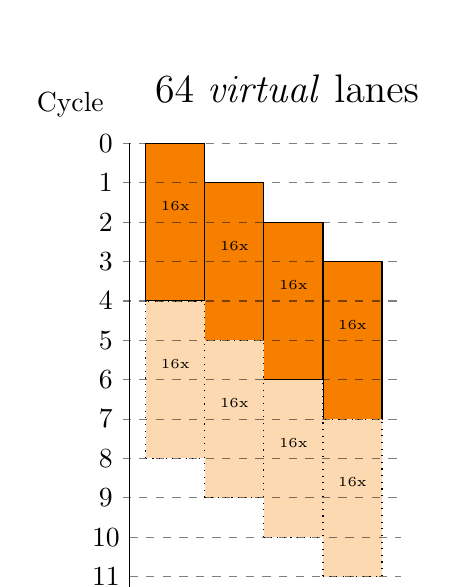
\begin{tikzpicture}
	\tikzstyle{simdbox}=[minimum height = 2cm, minimum width = 0.75cm,right=10mm, rectangle, draw=black, fill=color0]

	\foreach \x in {0,...,3}{
		\node[simdbox, label={[yshift=0.2cm]center:\tiny 16x}] (lanes\x) at (0.75cm * \x, -0.5cm * \x) {};
	}

	\foreach \x in {0,...,3}{
		\node[simdbox, dotted, fill=color0!30!white, label={[yshift=0.2cm]center:\tiny 16x}] (lanes2\x) at (0.75cm * \x, -2cm - 0.5cm * \x) {};
	}

	\node[right=10mm] (description) at (0cm, 1.7cm) {\Large 64 \emph{virtual} lanes};
	\node[right=10mm] (cycle-description) at (-1.5cm, 1.5cm) {Cycle};

	\foreach \x in {0,...,11}{
		\node[] (cycle\x) at (0.5cm, 1cm - 0.5cm * \x) {\x};
		\draw[dashed, opacity=0.5] (cycle\x) -- ++(3.75cm, 0cm);
	}

	\draw[->] (0.8cm, 1cm) -- ++(0cm, -0.25cm - 11 * 0.5cm);
\end{tikzpicture}
}

%\end{textblock*}
\begin{textblock*}{5cm}(11.7cm,2cm)
\scalebox{0.6}{
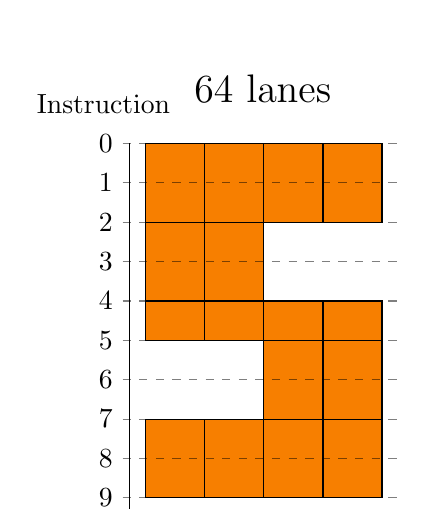
\begin{tikzpicture}
	\tikzstyle{simdbox}=[minimum height = 1cm, minimum width = 0.75cm,right=10mm, rectangle, draw=black, fill=color0]

	\foreach \x in {0,...,3}{
		\node[simdbox] at (0.75cm * \x, 0.5cm) {};
	}

	\node[simdbox] at (0.75cm * 0, -0.5cm) {};
	\node[simdbox] at (0.75cm * 1, -0.5cm) {};
	\foreach \x in {0,...,3}{
		\node[simdbox, minimum height=0.5cm] at (0.75cm * \x, -1.25cm) {};
	}

	\node[simdbox] at (0.75cm * 2, -2cm) {};
	\node[simdbox] at (0.75cm * 3, -2cm) {};
	\foreach \x in {0,...,3}{
		\node[simdbox] at (0.75cm * \x, -3cm) {};
	}

	\node[right=10mm] (description) at (0.5cm, 1.7cm) {\Large 64 lanes};
	\node[right=10mm] (cycle-description) at (-1.5cm, 1.5cm) {Instruction};

	\foreach \x in {0,...,9}{
		\node (cycle\x) at (0.5cm, 1cm - 0.5cm * \x) {\x};
		\draw[dashed, opacity=0.5] (cycle\x) -- ++(3.75cm, 0cm);
	}

	\draw[->] (0.8cm, 1cm) -- ++(0cm, -0.25cm - 9 * 0.5cm);
\end{tikzpicture}
}
\captionof{figure}{Executing an \emph{if-else} on SIMD units with an \emph{EXEC mask}}
\label{fig:gpu-simd-condition}

\end{textblock*}
% Difference for for-loops
% CPU: SIMD operation for subsequent iteranions
% GPU: SIMD for multiple threads
\end{frame}

%%%%%%%%%%%%%%%%%%%%%%%%%%%%%%%%%%%%%%%%%%%%%%%%%%%%%%%%%%%%%%%%%%%%%%%%%%%%%%%%%%%%%
{\framelogo{\centering\includesvg[width=3cm]{figures/Vulkan_API_logo.svg}}
\begin{frame}{Vulkan}{Software}
\begin{itemize}
	\item Graphics and compute standard for GPUs
	\item Shaders are loaded in SPIR-V
	\item Compilation to ISA happens in driver
\end{itemize}
\end{frame}}

%%%%%%%%%%%%%%%%%%%%%%%%%%%%%%%%%%%%%%%%%%%%%%%%%%%%%%%%%%%%%%%%%%%%%%%%%%%%%%%%%%%%%
\begin{frame}{\only<-2>{Workflow}\only<3>{Current State}\only<4->{This Thesis}}{Profile-Guided Optimization}
\begin{center}
\begin{tikzpicture}
	\tikzstyle{box}=[minimum height = 1cm, minimum width = 1.5cm, right=10mm, align=center, rectangle, draw=black]
	\tikzstyle{boundingbox}=[draw=green, thick, rounded corners, inner sep=0.2cm]

	\node[box] (compile) at (0cm, 0cm) {\scriptsize Compile};
	\node[box, right=of compile] (run) {\scriptsize Profile};
	\node[box, right=of run] (compile2) {\scriptsize Compile};
	\node[box, right=of compile2] (run2) {\scriptsize Run};

	\node[above=of compile] (code) {\includesvg[height=1.2cm]{figures/file.svg}};
	\node[above=0.1cm of code] {\scriptsize Code};
	\node[below=of run] (data) {\includesvg[height=1.2cm]{figures/file.svg}};
	\node[below=0.1cm of data] (datal) {\scriptsize Data};

	\draw[->] (compile) -- (run);
	\draw[->] (run) -- (compile2);
	\draw[->] (compile2) -- (run2);
	\draw[->] (code) -- (compile);
	\draw[->] (code) -| (compile2);
	\draw[->] (run) -- (data);
	\draw[->] (data) -| (compile2);

	\node[align=center, rotate=-30, text=color2, above right=0.5cm and -0.5cm of run2] (faster) {\footnotesize Faster! 🎉};

	\visible<2->{
		\node[boundingbox, fit=(run)(compile2)(datal)] (new) {};
		\node[boundingbox, fit=(faster)] (new2) {};
		\node[below left=-0.45cm and -1.9cm of new] (newl) {\scriptsize \textbf{Now possible}};
	}
\end{tikzpicture}
\end{center}

\end{frame}

%%%%%%%%%%%%%%%%%%%%%%%%%%%%%%%%%%%%%%%%%%%%%%%%%%%%%%%%%%%%%%%%%%%%%%%%%%%%%%%%%%%%%
\begin{frame}{Basic Block Counting}
	\centering
	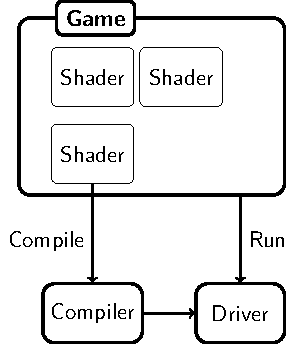
\includegraphics{figures/bb-count-overview-figure0.pdf}
\end{frame}

%%%%%%%%%%%%%%%%%%%%%%%%%%%%%%%%%%%%%%%%%%%%%%%%%%%%%%%%%%%%%%%%%%%%%%%%%%%%%%%%%%%%%
\framelogo{\centering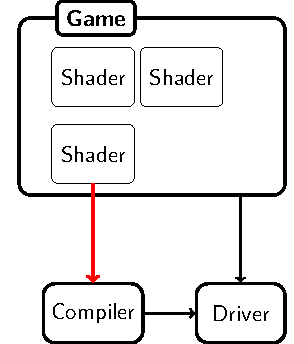
\includegraphics[width=3cm]{figures/bb-count-overview-figure1.pdf}}
\begin{frame}[fragile]{Basic Block Counting}{GLSL/SPIR-V}
\begin{itemize}
	\item GLSL gets precompiled to SPIR-V
	\item SPIR-V is passed to driver
\end{itemize}

\begin{lstlisting}
if (inputPos.x < 0.5) {
	outColor = vec4(1.0, 0.0, 0.0, 1.0);
} else {
	outColor = vec4(0.0, 0.0, 1.0, 1.0);
}
\end{lstlisting}
\end{frame}
\framelogo{}

%%%%%%%%%%%%%%%%%%%%%%%%%%%%%%%%%%%%%%%%%%%%%%%%%%%%%%%%%%%%%%%%%%%%%%%%%%%%%%%%%%%%%
{\framelogo{\centering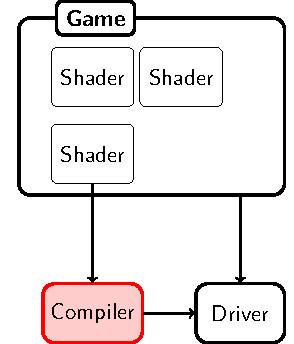
\includegraphics[width=3cm]{figures/bb-count-overview-figure2.pdf}}
\begin{frame}{Basic Block Counting}{CFG}
	\centering
	\begin{tikzpicture}
	\tikzstyle{box}=[minimum height=0.8cm, minimum width=0.8cm, rectangle, draw=black]

	\node[box] (a) at (0cm, 0cm) {A};
	\node[box] (b) at (-1cm, -1.5cm) {B};
	\node[box] (c) at (1cm, -1.5cm) {C};
	\node[box] (d) at (0cm, -3cm) {D};

	\draw[->] (a) -- (b);
	\draw[->] (a) -- (c);
	\draw[->] (b) -- (d);
	\draw[->] (c) -- (d);

	\visible<2>{
		\node[text=highlight] (insert) at (4cm, -1.5cm) {Insert counters here};
		\draw[->] (insert.west)++(0cm, 0.2cm) -- (a);
		\draw[->] (insert.west) -- (c);
	}

	\visible<3->{
		\node[align=center] at (3cm, -1.5cm) {Structurize\\$\Rightarrow$};

		\node[box] (a2) at (5cm, 1.5cm) {A};
		\node[box] (b2) at (6cm, 0cm) {B};
		\node[box, align=center] (a2') at (5cm, -1.5cm) {flip\\mask};
		\node[box] (c2) at (6cm, -3cm) {C};
		\node[box] (d2) at (5cm, -4.5cm) {D};

		\draw[->] (a2) -- (b2);
		\draw[->] (a2) -- (a2');
		\draw[->] (b2) -- (a2');
		\draw[->] (a2') -- (c2);
		\draw[->] (a2') -- (d2);
		\draw[->] (c2) -- (d2);
	}

	\visible<4>{
		\node[align=left, text=highlight] (insert) at (7.7cm, 1.5cm) {Insert\\wave-counters\\here};
		\draw[->] (insert) -- (a2);
		\draw[->] (insert) -- (b2);
		\draw[->] (insert) -- (c2);
	}
\end{tikzpicture}

\end{frame}}

%%%%%%%%%%%%%%%%%%%%%%%%%%%%%%%%%%%%%%%%%%%%%%%%%%%%%%%%%%%%%%%%%%%%%%%%%%%%%%%%%%%%%
%\framelogo{\centering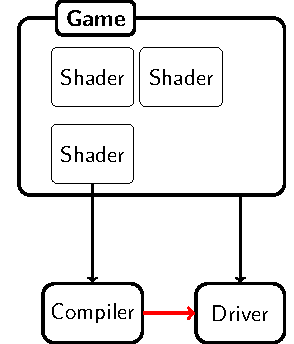
\includegraphics[width=3cm]{figures/bb-count-overview-figure3.pdf}}
%\begin{frame}[fragile]{Basic Block Counting}{ELF}
%\begin{itemize}
%	\item ELF file contains metadata and sections for counters
%\end{itemize}

%\begin{lstlisting}[language=erlang, morekeywords={text, rel, __llvm_prf_cnts, __llvm_prf_data}]
%.text
%	<code>

%.rel.text
%	<relocations for counter-pointers>

%__llvm_prf_cnts
%	<zero initialized counters>

%__llvm_prf_data
%	<metadata>
%\end{lstlisting}
%\end{frame}
%\framelogo{}

%%%%%%%%%%%%%%%%%%%%%%%%%%%%%%%%%%%%%%%%%%%%%%%%%%%%%%%%%%%%%%%%%%%%%%%%%%%%%%%%%%%%%
{\framelogo{\centering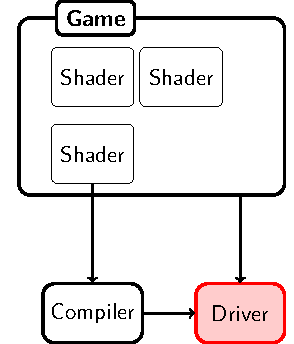
\includegraphics[width=3cm]{figures/bb-count-overview-figure4.pdf}}
\begin{frame}{Basic Block Counting}{Save Counter}
% This means the GPU pipeline, not LLVM!
\begin{itemize}
	\item Counters are saved when the pipeline is destroyed and every \SI{10}{\second}
	\item Fetch counters from GPU memory
	\item Write counters and metadata to file
	%\item LLVM runtime library is linked into driver
\end{itemize}
\end{frame}}

%%%%%%%%%%%%%%%%%%%%%%%%%%%%%%%%%%%%%%%%%%%%%%%%%%%%%%%%%%%%%%%%%%%%%%%%%%%%%%%%%%%%%
{\framelogo{\centering\includesvg[width=2cm]{clipart/RacingFlag.svg}}
\begin{frame}{Basic Block Counting}{Result}
\begin{itemize}
	\item Declares pixel shader as \emph{hot} and vertex shader as \emph{unlikely}
	\item Changes basic block ordering
\end{itemize}
\end{frame}}

%%%%%%%%%%%%%%%%%%%%%%%%%%%%%%%%%%%%%%%%%%%%%%%%%%%%%%%%%%%%%%%%%%%%%%%%%%%%%%%%%%%%%
{\framelogo{\centering\includesvg[width=2cm]{clipart/RacingFlag.svg}}
\begin{frame}{Basic Block Counting}{Result}
{\color{secondary}Dota 2: No change apart from compilation speed on first run}
\begin{tikzpicture}
\pgfplotsset{every non boxed y axis/.append style={y axis line style=-}}
\begin{axis}[
	xbar=0.2cm,
	xlabel={{\color{secondary}$\blacktriangleleft$} Time per frame [\SI{}{\milli\second}], less is better},
	symbolic y coords={Normal,PGO},
	xmin=0,
	xmax=30,
	ytick=data,
	nodes near coords, nodes near coords align={horizontal},
	bar width=0.5cm,
	grid=both,
	axis lines=left,
	enlarge y limits=0.5,
	y=1cm,
	%legend style={at={(1,1)},anchor=north east}
]

\addplot [
	fill=secondary,
	%only marks,
	%mark = +,
	%mark size = 1.5,
	%error bars/.cd,
	%y dir = both,
	%y fixed = 0.08
] coordinates {(24.15,Normal) (24.15,PGO)};
\end{axis}
\end{tikzpicture}
\ \\

{\color{secondary}Ashes of the Singularity: \SI{60.007 \pm 0.004}{\milli\second} vs \SI{60.009 \pm 0.003}{\milli\second}}
\begin{tikzpicture}
\pgfplotsset{every non boxed y axis/.append style={y axis line style=-}}
\begin{axis}[
	xbar=0.2cm,
	xlabel={{\color{secondary}$\blacktriangleleft$} Time per frame [\SI{}{\milli\second}], less is better},
	symbolic y coords={Normal,PGO},
	xmin=0,
	xmax=75,
	ytick=data,
	nodes near coords, nodes near coords align={horizontal},
	nodes near coords style={/pgf/number format/precision=5},
	bar width=0.5cm,
	grid=both,
	axis lines=left,
	enlarge y limits=0.5,
	y=1cm,
]

\addplot [
	fill=secondary,
] coordinates {(60.007,Normal) (60.009,PGO)};
\end{axis}
\end{tikzpicture}
\end{frame}}

%%%%%%%%%%%%%%%%%%%%%%%%%%%%%%%%%%%%%%%%%%%%%%%%%%%%%%%%%%%%%%%%%%%%%%%%%%%%%%%%%%%%%
\begin{frame}{My Work}
\begin{itemize}
	\item Enable atomic basic block counters in LLVM
	\item Implement ELF loading and relocations in AMDVLK
	\item Write result files from driver
	\item Apply PGO per wave instead of per thread
	\item Fix bugs in LLVM (with PGO on GPUs)
\end{itemize}
\end{frame}

%%%%%%%%%%%%%%%%%%%%%%%%%%%%%%%%%%%%%%%%%%%%%%%%%%%%%%%%%%%%%%%%%%%%%%%%%%%%%%%%%%%%%
{\framelogo{\centering\includesvg[width=2cm]{clipart/Map.svg}}
\begin{frame}{Future Work}
\begin{itemize}
	\item Find dynamically uniform variables
	\item Create some interesting statistics, e.g. unused basic blocks, uniform branches
	\item More benchmarks
	\item (More optimizations)
\end{itemize}
\end{frame}}

%%%%%%%%%%%%%%%%%%%%%%%%%%%%%%%%%%%%%%%%%%%%%%%%%%%%%%%%%%%%%%%%%%%%%%%%%%%%%%%%%%%%%
\begin{frame}{Dead Code}{Ashes of the Singularity}
\begin{tikzpicture}
\begin{axis}[
	xlabel={\#BBs in a shader},
	ylabel={\#Shaders},
	ymax=35,
	grid=both,
	axis lines=left,
]
	
\addplot [
	fill=secondary,
] table {data/ashes_bbs.txt}
\closedcycle;
\end{axis}
\end{tikzpicture}
\begin{tikzpicture}
\begin{axis}[
	xlabel={\#BBs in a shader},
	ylabel={Unused code [$\%$]},
	ymax=0.19,
	yticklabel style={ /pgf/number format/fixed, /pgf/number format/precision=2},
	grid=both,
	axis lines=left,
]
	
\addplot [
	fill=secondary,
] table {data/ashes_dead.txt};
\end{axis}
\end{tikzpicture}
\end{frame}

%%%%%%%%%%%%%%%%%%%%%%%%%%%%%%%%%%%%%%%%%%%%%%%%%%%%%%%%%%%%%%%%%%%%%%%%%%%%%%%%%%%%%
\begin{frame}{Dead Code}{Dota}
\begin{tikzpicture}
\begin{axis}[
	xlabel={\#BBs in a shader},
	ylabel={\#Shaders},
	ymax=35,
	grid=both,
	axis lines=left,
]
	
\addplot [
	fill=secondary,
] table {data/dota_bbs.txt}
\closedcycle;
\end{axis}
\end{tikzpicture}
\begin{tikzpicture}
\begin{axis}[
	xlabel={\#BBs in a shader},
	ylabel={Unused code [$\%$]},
	%ymax=0.19,
	yticklabel style={ /pgf/number format/fixed, /pgf/number format/precision=2},
	grid=both,
	axis lines=left,
]

\addplot [
fill=secondary,
] table {data/dota_dead.txt}
\closedcycle;
\end{axis}
\end{tikzpicture}
\end{frame}

%%%%%%%%%%%%%%%%%%%%%%%%%%%%%%%%%%%%%%%%%%%%%%%%%%%%%%%%%%%%%%%%%%%%%%%%%%%%%%%%
\begin{tumplainframe}{Thanks!}
\begin{center}
	\Huge Questions?
\end{center}
\end{tumplainframe}

\end{document}
